\section{Splines Catmull-Rom}

A curva de splines Catumull-Rom para dados pontos de controlo $P_{0}, P_{1}, P_{2} e P_{3}$, está definida de modo a que a tangente em cada ponto $P_{i}$ possa ser encontrada através da diferença entre os seus pontos vizinhos $P_{i-1}$ e $P_{i+1}$

\begin{center}
 	
 	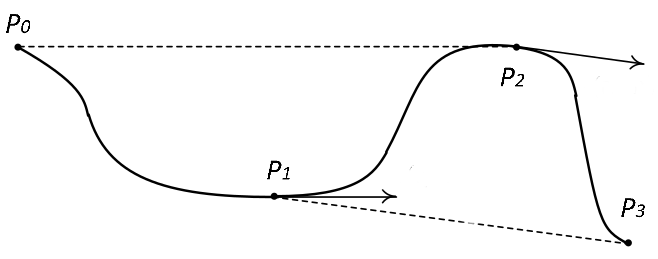
\includegraphics[scale=0.5,keepaspectratio]{resources/catmullDeriv.png}
 	\captionsetup{type=figure, width=0.8\linewidth}
	\caption{Spline Catmull-Rom para os pontos $P_{0}, P_{1}, P_{2} e P_{3}$}
\label{fig:ssec1:diagram:plane:to:sphere} 
\end{center}

Esta curva spline pode ser escrita em forma de matriz:

\begin{equation}
\frac{P_{2}-P_{0}}{2} = P_{1}^{'} = P^{'}(0) = c  \nonumber
\end{equation}
\begin{equation}
P_{1} = P(0) = d 		\nonumber
\end{equation}
\begin{equation}
P_{2}=P(1)=a+b+c+d 		\nonumber
\end{equation}
\begin{equation}
\frac{P_{3}-P_{1}}{2} = P_{2}^{'} = P^{'}(1) = 3a+2b+c 
\end{equation}


o que é equivalante a:

\begin{equation}
P_{0} = a+b-c+d 		\nonumber
\end{equation}
\begin{equation}
P_{1} = P{0} = d 		\nonumber
\end{equation}
\begin{equation}
P_{2}=P(1)=a+b+c+d 		\nonumber
\end{equation}
\begin{equation}
P_{3}=6a+4b+2c+1
\end{equation}

este conjunto de equações pode-se representar na seguinte operação de matrizes:

P=$\begin{bmatrix}
		       P_{0}           \\[0.3em]
		       P_{1}   \\[0.3em]
		       P_{2} \\[0.3em]
		       P_{3}
		     \end{bmatrix}$ = $\begin{bmatrix}
		      					 1 & 1 & -1 & 1           \\[0.3em]
		       					 0 & 0 & 0 & 1   \\[0.3em]
		       					 1 & 1 & 1 & 1 \\[0.3em]
		      					 6 & 4 & 2 & 1
		     					\end{bmatrix}$  $\begin{bmatrix}
		       									a_{x} & a_{y} & a_{z}    \\[0.3em]
		     								  	b_{x} & b_{y} & b_{z}    \\[0.3em]
		       									c_{x} & c_{y} & c_{z}    \\[0.3em]
		       									d_{x} & d_{y} & d_{z} 
		     					\end{bmatrix}$   = $C * A$

Estes cálculos até agora demonstrados irão ser aplicados algoritmicamente no programa da seguinte maneira:

$\begin{bmatrix}
       x(u) & y(u) & z(u)           \\[0.3em]
\end{bmatrix}$ = 
$\begin{bmatrix}
       t^{3} & t^{2} & t & 1          \\[0.3em]
		\end{bmatrix}$ $\begin{bmatrix}
		      					 -0.5 & 1.5 & -1.5 & 0.5           \\[0.3em]
		       					 1 & -2.5 & 2 & -0.5   \\[0.3em]
		       					 -0.5 & 0 & 0.5 & 0 \\[0.3em]
		      					 0 & 1 & 0 & 0
		     					\end{bmatrix}$ $\begin{bmatrix}
         							    P_{0}           \\[0.3em]
       									P_{1}   \\[0.3em]
       									P_{2} \\[0.3em]
       									P_{3}
     \end{bmatrix}$